\documentclass{article}

\PassOptionsToPackage{numbers,sort&compress}{natbib}
\usepackage{neurips_2026}

\usepackage[utf8]{inputenc}
\usepackage[T1]{fontenc}
\usepackage{hyperref}
\usepackage{url}
\usepackage{booktabs}
\usepackage{multirow}
\usepackage{amsfonts}
\usepackage{amsmath}
\usepackage{amssymb}
\usepackage{microtype}
\usepackage{xcolor}
\usepackage{graphicx}
\usepackage{tikz}
\usetikzlibrary{arrows.meta,positioning,fit,backgrounds}

\hypersetup{hidelinks}

\graphicspath{{figures/}{../figures/}}

% Compact float layout. Page geometry is the unmodified NeurIPS style.
\makeatletter
\setlength{\@neuripsabovecaptionskip}{4\p@}
\makeatother
\setlength{\textfloatsep}{9pt plus 2pt minus 2pt}
\setlength{\intextsep}{8pt plus 2pt minus 2pt}
\setlength{\floatsep}{8pt plus 2pt minus 2pt}
\renewcommand{\arraystretch}{0.96}

\newcommand{\nem}{\textsc{NemChua}}
\newcommand{\Dobs}{D_{\mathrm{obs}}}
\newcommand{\Hyp}{\mathcal{H}}

\title{\nem: What Does an LLM Proposer Add?\\ An Audit in Active Causal Discovery}

\author{%
  Anonymous Author(s) \\
  Affiliation \\
  Address \\
  \texttt{email} \\
}

\begin{document}

\maketitle

\begin{abstract}
Scientific agents increasingly pair a generative proposer with a mechanical verifier, but a verifier
good enough to rescue weak proposals also makes end-to-end accuracy a poor measure of what the
proposer contributed. We study this attribution problem in active causal discovery through \nem{},
which asks an LLM to flag likely errors in a PC-estimated skeleton and delegates every remaining
decision to a bounded model-based pipeline: candidates receive BIC weights, interventions are chosen
by Monte Carlo expected information gain, and the weights are updated by exact interventional
likelihoods. \nem{} reaches $0.956$ directed-edge F1 on $80$ paired synthetic instances against
$0.874$ for PC+greedy+Meek, the strongest external baseline we include. Controls dissolve most of
that apparent contribution. Replacing the model with an editor that draws edits uniformly at random
costs almost nothing, and across five proposers a $4.2\times$ spread in edit precision moves final
F1 by $0.026$ without preserving the ordering. Removing the likelihood update or the candidate-budget
guard costs far more than changing the proposer, and the guard is exactly free for a perfect
proposer. Auditing the proposals explains why: our prompt stated that a nonzero partial correlation
given all other variables implies adjacency, which is false for a DAG, and the models' wrong
additions concentrate on precisely the co-parent pairs that error invites --- more so the more
capable the model. Capability was being spent on complying with a misspecified interface. Random,
no-proposal, and oracle controls, together with an audit of the proposals themselves, are what a
propose-and-verify result needs before its success can be credited to its generator.
\end{abstract}

\section{Introduction}
\label{sec:intro}

Propose-and-verify has become a natural architecture for LLM scientific agents: the model generates
candidate hypotheses, trusted machinery evaluates them, and only candidates that survive this
evaluation influence the answer. This division of labor is appealing because a strong verifier can
bound the damage caused by an unreliable generator, but the same protection complicates scientific
attribution. An end-to-end comparison against a baseline that contains neither component
cannot reveal whether the model supplied useful hypotheses, whether the verifier supplied a better
decision rule, or whether the interaction between them mattered.

Resolving that ambiguity requires a counterfactual that is often absent from evaluations of
scientific agents: the downstream machinery must remain fixed while the learned proposer is replaced
by a source with no domain knowledge. If both systems perform similarly, the result may still
validate the architecture, but it cannot support the stronger claim that the model understood the
domain. Our experiments instantiate this comparison directly and then trace the proposal signal
through every subsequent stage to determine where, if anywhere, model-specific information changes
the final answer.

Active causal discovery provides an unusually transparent setting for this audit because its central
ambiguity has an experimental resolution. Observational data may leave $A \to B$ indistinguishable
from $B \to A$, whereas a carefully chosen intervention can resolve the direction. An agent receives
an observational sample, a small experimental budget, and
the task of returning the directed graph. At the graph sizes studied here, candidate generation and
model-based updating remain inspectable graph by graph, allowing us to observe not only what the LLM
proposed but also whether that proposal entered the candidate set, survived scoring, and altered the
submitted graph. The main benchmark names variables $X_0 \dots X_{d-1}$ to remove semantic cues,
while a separate condition restores published labels and a domain description to probe the distinct
setting in which prior knowledge might supplement limited data.

The resulting evaluation treats system quality and proposer value as related but separate questions.
A protective decision layer may transform weak proposals into strong final answers while
simultaneously erasing differences among generators. We therefore follow each proposal from its
edit-level correctness, through candidate-set coverage and ranking, to its effect on the submitted
graph. This view asks not only whether the assembled system works, but whether its behavior would
have changed had the language model contributed less informative proposals.

\paragraph{Contributions.}
\begin{itemize}\itemsep1pt
\item \textbf{An auditable proposal interface.} We isolate the LLM to skeleton edits and make the
remaining candidate search, scoring, experiment selection, and likelihood update mechanical. This
turns the path from proposal to final graph into a sequence of measurable bottlenecks
(Section~\ref{sec:method}).
\item \textbf{Controls that reassign the credit.} We compare no edits, uniformly random edits,
LLM edits, and oracle edits inside the same downstream architecture. The system performs well, but
the random control nearly matches the LLMs, while decision-layer ablations explain far more of the
final accuracy than model choice (Sections~\ref{sec:main}--\ref{sec:mechanism}).
\item \textbf{A scoped account of when proposal content may matter.} Sample-size sweeps and an
exploratory semantic condition identify data scarcity and meaningful prompt context as plausible
boundary conditions. We also state the statistical and control-design limitations that prevent
these observations from supporting a broader claim about LLM causal knowledge
(Section~\ref{sec:when}).
\end{itemize}

\section{Background: from observation to intervention}
\label{sec:background}

We summarize only the concepts needed to interpret the experiments here and give the formal model
in Appendix~\ref{app:background}. Suppose $d$ observed variables are generated by an unknown
directed acyclic graph (DAG), with each variable a noisy linear function of its parents.
Observational data can reveal which pairs are directly connected, forming the graph's
\emph{skeleton}, and can orient some but not all of those connections; the observationally
indistinguishable DAGs constitute a Markov equivalence class. Interventions supply the missing
asymmetry: forcing $X_a$ to an unusual value can change its descendants, and among the variables
adjacent to $a$, only its children respond. A sequence of such local comparisons can therefore
resolve directions that observation alone leaves ambiguous.

An active discovery system must decide both which graphs remain plausible and which interventions
will best distinguish among them. Its candidate set $\Hyp$ imposes a hard epistemic ceiling, since
no experimental policy can recover the true graph after that graph has been excluded. We construct
the initial skeleton with PC, which removes an adjacency when the data support a conditional
independence. Finite-sample tests can miss genuine dependencies, so the resulting estimate is strong
but incomplete: PC attains skeleton F1 $0.947$ on our main instances, while its estimated equivalence
class contains the true DAG only $45\%$ of the time. This combination creates a meaningful proposal
task. There is enough statistical structure to anchor the search, but also enough residual error for
a proposer to expand the set of graphs that the decision layer can consider.

\section{Method}
\label{sec:method}

\nem{} separates proposal from decision authority across the stages in Figure~\ref{fig:method}. The
language model acts only once, before any intervention is collected, and can alter the search only by
naming suspected skeleton errors. Candidate construction, graph scoring, experiment selection,
evidence accumulation, and final submission then proceed without further model input. This boundary
makes a proposal consequential only through the hypotheses that it adds to or displaces from the
finite candidate set.

\begin{figure}[t]
\centering
\resizebox{0.97\linewidth}{!}{%
\begin{tikzpicture}[
  font=\small,
  box/.style={draw, rounded corners=2pt, align=center, inner sep=4pt, minimum height=9mm},
  llm/.style={box, fill=blue!8, draw=blue!55},
  det/.style={box, fill=black!5, draw=black!45},
  env/.style={box, fill=orange!10, draw=orange!60},
  ar/.style={-{Latex[length=2mm]}, thick, draw=black!60}
]
  \node[det] (obs) at (0,0) {$\Dobs$\\ \scriptsize observations};
  \node[det] (pc) at (2.2,0) {PC\\ \scriptsize skeleton $S$};
  \node[llm] (llm) at (5.0,0) {\textbf{LLM proposer}\\ \scriptsize ``which adjacencies\\ \scriptsize did PC get wrong?''};
  \node[det] (enum) at (8.3,0) {enumerate\\ \scriptsize orientations of $S$\\ \scriptsize and of each edit};
  \node[det] (bic) at (11.4,0) {BIC score\\ \scriptsize approximate weights $w$ over $\Hyp$};

  \node[det] (eig) at (11.4,-2.3) {max EIG\\ \scriptsize pick target $a_t$};
  \node[env] (env) at (8.3,-2.3) {environment\\ \scriptsize $\mathrm{do}(X_{a_t}\!=\!v)$};
  \node[det] (bayes) at (5.0,-2.3) {likelihood update\\ \scriptsize fitted Gaussian models};
  \node[det] (out) at (1.6,-2.3) {submit\\ \scriptsize $\arg\max_h w_h$};

  \draw[ar] (obs) -- (pc);
  \draw[ar] (pc) -- (llm);
  \draw[ar] (llm) -- (enum);
  \draw[ar] (enum) -- (bic);
  \draw[ar] (bic) -- (eig);
  \draw[ar] (eig) -- (env);
  \draw[ar] (env) -- (bayes);
  \draw[ar] (bayes) -- (out);
  \draw[ar] (bayes) -- ++(0,1.15) -| (bic);
  \node[anchor=west, font=\scriptsize, text=blue!60] at (3.15,0.95)
        {at most 4 removals and 4 additions, once per episode};
  \node[draw=black!45, dashed, rounded corners=2pt, fill=white, inner sep=3pt,
        font=\scriptsize, align=center, text=black!70] (guard) at (8.3,-1.17)
        {\textbf{the guard:} half of $|\Hyp|$ is held for orientations of PC's\\
         \emph{unedited} skeleton, limiting candidate crowd-out};
  \draw[draw=black!40, dashed] (guard) -- (enum);
  \node[anchor=west, font=\scriptsize, text=black!55] at (0.6,-3.3)
        {the model never sees interventional data, and never writes an edge};
\end{tikzpicture}}
\caption{\nem{}. The LLM contributes one list of suspected adjacency errors and nothing else; the
candidate set, the scores, the experiment choice, the belief update and the submitted graph are
all mechanical. Section~\ref{sec:credit} replaces the blue box with a random editor and with an
oracle editor, holding everything else fixed.}
\label{fig:method}
\end{figure}

\paragraph{1. Propose a local correction.}
The model receives the correlation matrix, the partial correlation of every pair given all other
variables, PC's adjacency set, and the currently non-adjacent pairs. Its single tool call may remove
or add at most four adjacencies of each kind, after which the model leaves the loop and never observes
interventional data. This interface deliberately asks for a local correction rather than a complete
graph, but the statistical guidance in the executed prompt is flawed: it describes non-zero
full-order partial correlation as equivalent to direct adjacency. Conditioning on a collider such as
$X_1 \to X_3 \leftarrow X_2$ can instead make $X_1$ and $X_2$ dependent even though they are not
adjacent. Because Appendix~\ref{app:prompts} reproduces and audits the executed prompt, the proposer
results can be interpreted accurately as evidence about this statistically misspecified
interface, not as a general test of whether LLMs can propose causal structure from valid evidence.

\paragraph{2. Expand the neighborhood without discarding the anchor.}
Let $S$ denote PC's skeleton. We construct its all-edits variant and every single-edit variant, then
enumerate acyclic orientations exhaustively when the space is small and by sampling otherwise.
Least-squares fits and linear-Gaussian BIC scores on the observational sample define
$w_h \propto \exp(-\tfrac12\mathrm{BIC}_h)$ over a retained set $\Hyp$ of at most $48$ DAGs. These
normalized scores form an approximate belief over a truncated hypothesis set rather than an exact
structure posterior, so proposal and pruning determine what the later evidence can possibly recover.

To prevent edited variants from consuming the entire candidate budget, the guard first reserves
half of $\Hyp$ for the best-scoring orientations of the unedited skeleton. Edited orientations fill
the remaining slots, with unused capacity backfilled from the original skeleton. This reservation
reduces displacement without eliminating it: an unedited-only arm may use all $48$ slots for the
base skeleton, whereas a guarded edit arm guarantees only half of them. The protection offered by
the guard is therefore an empirical property of this budget and search procedure, not a formal
guarantee that accepting a proposal is cost-free (Section~\ref{sec:mechanism}).

\paragraph{3. Choose experiments, update the weights, and submit.}
For each variable whose orientation remains ambiguous under $w$, we estimate the expected
information gain about the hypothesis index from $12$ Monte Carlo outcomes and intervene on the
maximizer. Although the objective is the standard Bayesian design criterion, its computed value is
an approximation under fitted parameters and a finite candidate set. Each observed interventional
batch is then evaluated under the candidates' mutilated linear-Gaussian likelihoods, which are
available in closed form conditional on those fitted parameters. The weights are multiplied and
renormalized after every experiment, and the loop continues until the budget is exhausted or
$\max_h w_h > 0.999$, at which point the highest-weight retained graph is submitted.

\section{Experimental setup}
\label{sec:setup}

\paragraph{Instances.}
The main benchmark contains twenty accepted instances at each of four graph sizes,
$d \in \{4,6,8,10\}$ with $|E|=d$, yielding $80$ instances shared across all arms. Acceptance
requires a connected skeleton and a nontrivial, distributed orientation problem: the equivalence
class must contain at least two undirected edges, those edges cannot all meet at one node, and at
least one intervention must be necessary. Edge coefficients are drawn from
$(-2,-0.5)\cup(0.5,2)$, bounded away from zero so that faithfulness violations are not generic.
Unless otherwise noted,
each instance supplies $n_{\mathrm{obs}}=300$ observational
rows and $n_{\mathrm{int}}=150$ samples per intervention. The experimental budget is
$|I^*|+1$ for a minimum identifying set $I^*$, allowing $2.7$ interventions on average, and a random
permutation maps the variables to anonymous labels $X_0 \dots X_{d-1}$; Appendix~\ref{app:instances}
reports the complete difficulty ladder and its acceptance statistics.

\paragraph{Comparators and controls.}
Every arm runs on every instance, making the principal comparisons paired. Reference arms include
an oracle ceiling; \texttt{PC+greedy}, which intervenes on the highest-degree ambiguous node and
orients by a mean-shift test, with or without Meek closure; and \texttt{LLM-e2e}, which gives the
same models raw data and control of the full loop. The proposal-content controls retain \nem's
decision layer while changing only the source of its search neighborhood. The \texttt{no-edits}
arm uses PC's original skeleton, \texttt{random-edits} samples up to four removals from PC
adjacencies and four additions from currently non-adjacent pairs, and \texttt{perfect-edits} applies
up to four ground-truth errors of each kind. Because the random arm matches the permitted cap rather
than either model's realized edit count and uses a single seeded draw per instance, it should be read
as a weak shared control rather than a per-model randomization null. Additional arms supply PC's
equivalence class, complete DAGs written by the LLM, or random DAGs. Decision-layer ablations replay
the recorded LLM proposal and generally preserve candidate membership; the \texttt{no-guard}
ablation is the exception because its purpose is to let edited candidates compete for every slot.

\paragraph{Models, pairing, and proposal audit.}
We evaluate five proposers spanning roughly two orders of magnitude in price:
\texttt{qwen3-coder-30b}, \texttt{gpt-4o-mini}, \texttt{gpt-5.4-mini},
\texttt{claude-haiku-4.5}, and \texttt{gemini-3-flash}, all at temperature zero with forced tool
calls; Appendix~\ref{app:instances} lists the complete identifiers. The capability sweep runs on its
own cohort rather than on the main table's instances: $60$ instances at $d\in\{6,8,10\}$ with
$n_{\mathrm{obs}}{=}60$, chosen because the proposal channel is live only where the statistical
front-end is underpowered. Every table below states the cohort it uses, and numbers are comparable
across tables only within a cohort. Within an instance, every
mechanical ablation replays the same recorded proposal, preventing provider variability from
entering those contrasts. Error bars are $95\%$ confidence intervals over instances for arm means
and over paired differences for contrasts, while pairwise claims on the synthetic ladder use
two-sided Wilcoxon signed-rank tests with win and loss counts. The semantic study reuses each base
parameterization across five models, so pooled episode-level comparisons are descriptive rather than
independent confirmatory tests. To connect proposal behavior to downstream performance, we also
score every retained edit against the true skeleton: a removal is correct when PC introduced a
spurious adjacency, and an addition is correct when PC omitted a genuine one, so every reference to
``edits correct'' uses the post-sanitization changes that the pipeline actually receives.

\section{Results}
\label{sec:results}

\subsection{A strong system, followed by the control it needs}
\label{sec:main}

Viewed only at the system boundary, the main comparison in Table~\ref{tab:main} resembles a
conventional success story. \nem{} reaches $0.956$ directed F1 with \texttt{gpt-4o-mini} and $0.953$
with \texttt{qwen3-30b}, compared with $0.874$ for \texttt{PC+greedy+Meek}, the strongest external
baseline included here. For \texttt{gpt-4o-mini}, the paired gain is $0.082$ with a $95\%$ confidence
interval of $[0.041,0.127]$, and the trajectory in Figure~\ref{fig:main}(b) passes the baseline's
full-budget score after only two experiments. Despite this strong pooled result, the advantage is
concentrated at $d{=}4$, where PC produces its weakest skeleton, and falls to
$0.017$--$0.030$ when that level is excluded. The per-level results in
Appendix~\ref{app:scaling} therefore suggest that \nem{} repairs a pronounced local failure of the
statistical front-end rather than improving active discovery to the same degree across regimes.

The weak end-to-end rows serve a narrower purpose by revealing how strongly performance depends on
the interface through which a model acts. In all $80$ \texttt{gpt-4o-mini} episodes, the model
submits no directed edges even though it proposes an average of $2.79$ undirected edges. Every tool
call is valid and no parser repair is triggered, which rules out silent schema rejection and instead
indicates a systematic choice to leave proposed adjacencies unresolved. Asking the same models for
complete DAGs improves on this behavior but remains roughly $0.30$ F1 below the edit interface.
These comparisons establish that constraining model authority can improve the assembled system;
they do not, by themselves, establish that the proposal content is informative. The attribution
claim therefore rests on the controlled replacements considered next rather than on the unusually
weak end-to-end baseline.

\begin{table}[t]
\caption{Main results. $80$ paired instances per arm; directed F1 is reported as mean $\pm$ $95\%$
CI over instances, and the remaining columns report means only. Arms in the middle
block share \nem's decision layer and differ in the source of candidate graphs. The random editor
uses one seeded, cap-matched draw per instance, not a per-model realized-count match. Tokens and
calls are per episode.}
\label{tab:main}
\centering
\small
\setlength{\tabcolsep}{4.2pt}
\begin{tabular}{llcccccc}
\toprule
Arm & Model & directed F1 & skel.\ F1 & SHD & interv. & tokens & calls \\
\midrule
\multicolumn{8}{l}{\emph{reference and baselines}}\\
ground-truth ceiling & N/A & $1.000 \pm 0.000$ & $1.000$ & $0.00$ & $0.00$ & $0$ & $0$ \\
PC $+$ greedy & N/A & $0.868 \pm 0.041$ & $0.947$ & $1.14$ & $1.98$ & $0$ & $0$ \\
PC $+$ greedy $+$ \textsc{Meek} & N/A & $0.874 \pm 0.040$ & $0.947$ & $1.02$ & $1.81$ & $0$ & $0$ \\
LLM end-to-end & qwen3-30b & $0.202 \pm 0.038$ & $0.385$ & $9.86$ & $2.71$ & $50{,}924$ & $3.7$ \\
LLM end-to-end & gpt-4o-mini & $0.000 \pm 0.000$ & $0.138$ & $8.85$ & $2.65$ & $33{,}893$ & $3.6$ \\
\midrule
\multicolumn{8}{l}{\emph{where the skeleton edits come from (decision layer held fixed)}}\\
random DAGs & N/A & $0.298 \pm 0.050$ & $0.547$ & $8.82$ & $0.25$ & $0$ & $0$ \\
LLM writes whole DAGs & gpt-4o-mini & $0.649 \pm 0.050$ & $0.928$ & $2.74$ & $0.62$ & $1{,}339$ & $1.0$ \\
LLM writes whole DAGs & qwen3-30b & $0.669 \pm 0.059$ & $0.918$ & $2.73$ & $1.23$ & $2{,}315$ & $1.1$ \\
PC equivalence class & N/A & $0.868 \pm 0.043$ & $0.947$ & $1.00$ & $1.81$ & $0$ & $0$ \\
no edits (PC skeleton) & N/A & $0.901 \pm 0.036$ & $0.947$ & $0.88$ & $1.91$ & $0$ & $0$ \\
\textbf{random edits} & \textbf{none} & $\mathbf{0.951 \pm 0.022}$ & $0.967$ & $0.68$ & $2.41$ & $\mathbf{0}$ & $\mathbf{0}$ \\
\textbf{\nem} & qwen3-30b & $\mathbf{0.953 \pm 0.018}$ & $0.963$ & $0.61$ & $2.46$ & $1{,}807$ & $1.0$ \\
\textbf{\nem} & gpt-4o-mini & $\mathbf{0.956 \pm 0.018}$ & $0.969$ & $0.61$ & $2.41$ & $1{,}114$ & $1.0$ \\
oracle edits (main ceiling) & N/A & $0.999 \pm 0.003$ & $0.999$ & $0.01$ & $2.01$ & $0$ & $0$ \\
\bottomrule
\end{tabular}
\end{table}

\begin{figure}[t]
\centering
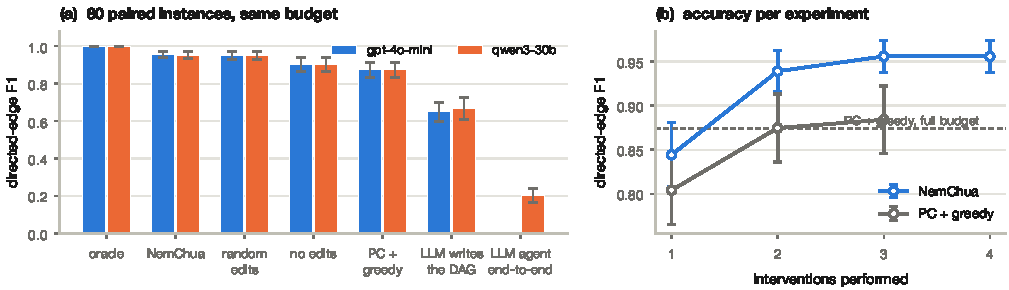
\includegraphics[width=\linewidth]{nemchua_f2_main.pdf}
\caption{(a) Arm means over $80$ paired instances. The random-edit control lies within $0.005$ of
both language models. (b) Accuracy after each experiment, carried forward once an arm stops;
\nem{} passes the included classical baseline's full-budget score on its second experiment.}
\label{fig:main}
\end{figure}

\subsection{Following proposal quality through the pipeline}
\label{sec:credit}

The attribution changes when \texttt{random-edits} replaces the LLM while leaving the entire
downstream pipeline intact. This deliberately simple editor reaches $0.951$, effectively level with
both language models, and all three edit arms improve on the unedited skeleton. Their common gain
suggests that much of the benefit comes from widening the search neighborhood around PC rather than
from selecting especially informative corrections. The oracle-edit arm continues to improve at
graph sizes where random and LLM edits do not, so adjacency repair remains a potentially valuable
channel; the learned proposers simply capture little of the available advantage under this
interface. Because the random arm is matched only to the edit cap and is represented by one seeded
draw, it cannot identify the exact marginal effect of model content. It supports the narrower but
still consequential conclusion that a simple model-free proposer reproduces the observed LLM score
at the implemented edit volume.

Evidence from the five-model sweep reinforces this interpretation without requiring the random
control to carry the entire argument. Edit precision changes by a factor of $4.2$ across models,
but downstream F1 remains within a $0.026$ band and no longer preserves the proposal-quality ordering
(Figure~\ref{fig:credit}(b)). The better models are demonstrably more selective and accurate at the
task assigned to them, which means that the flat final scores cannot be explained by an absence of
variation in proposal quality. Instead, the result indicates that the decision layer is insensitive
to much of the variation that enters through its proposal interface.

Because every intermediate stage is observable, we can identify where the pipeline loses sensitivity
to proposal quality. Stronger proposers recover more missing PC adjacencies and place the true DAG
in the candidate set more often, so their
advantage survives the initial expansion of the hypothesis space. Downstream, however, the best
directed graph available in the bounded set improves only modestly, and the graph ultimately selected
does not consistently reach even that within-set ceiling. With only $60$ observational rows, BIC
must discriminate among $48$ fitted candidates using weak evidence, after which a small intervention
budget must resolve the remaining uncertainty. The pipeline therefore separates two notions of
proposal value: better edits improve \emph{coverage} by admitting more relevant alternatives, but
they improve final accuracy only when scoring and experimental design can \emph{convert} that
coverage into a different decision. In these experiments, most of the proposal signal is lost during
that conversion.

\begin{figure}[t]
\centering
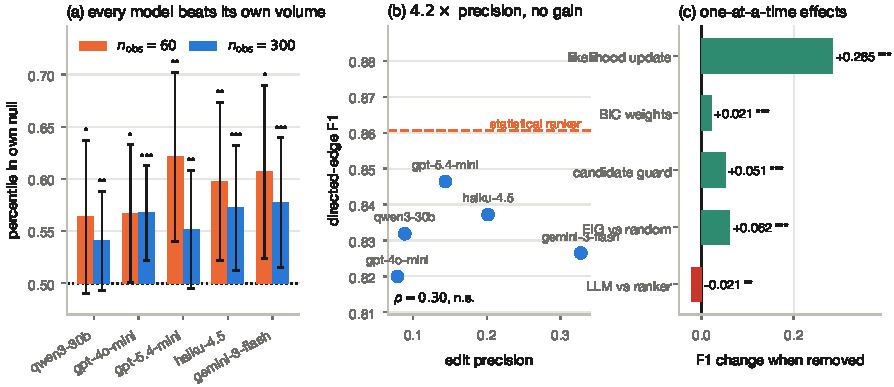
\includegraphics[width=\linewidth]{nemchua_f3_credit.pdf}
\caption{(a) The proposal-content ladder in the main regime: random edits are indistinguishable
from LLM edits, and both fall well short of oracle edits. (b) Five proposers at
$n_{\mathrm{obs}}{=}60$; the dashed line is the random-edit control. (c) One-at-a-time ablation
effects; these are sensitivities, not an additive decomposition, and do not sum. What each component is
worth, paired, in the main regime.}
\label{fig:credit}
\end{figure}

\label{sec:mechanism}
Once proposal identity becomes nearly interchangeable, the system's advantage over the classical
baseline must be explained by operations shared across proposers. The component ablations in
Table~\ref{tab:decision}, summarized alongside the proposal controls in
Figure~\ref{fig:credit}(c), reveal that the gain is distributed across the statistical decision
process rather than supplied by a single verification step. Removing the likelihood update costs
about $0.29$ F1 because the system continues to perform experiments while discarding the evidence
they produce, an effect roughly an order of magnitude larger than the spread across proposers.
Choosing intervention targets also matters relative to random selection, although a max-degree
heuristic nearly matches the Monte Carlo information-gain policy in this regime. BIC initialization
has a smaller effect than the update, but together these ablations show that the submitted graph
emerges from a sequence of approximate statistical decisions rather than from an exact verifier that
simply accepts or rejects an LLM guess.

Candidate-set construction contributes a different kind of value by limiting the damage a proposal
can cause before any experiment is evaluated. When the guard is removed, edited orientations compete
for every one of the $48$ slots and final F1 falls by roughly $0.05$. The true DAG survives in
$69\%$ of guarded candidate sets but only $24\%$ of their unguarded counterparts, with the random
editor showing the same qualitative pattern. By contrast, the oracle-edit arm is unchanged on these
instances, indicating that the reservation protects the system from poor proposals without a
measurable cost when the proposed correction is exact. This comparison explains why the guard is
more consequential here than model choice, while remaining an empirical result tied to the present
candidate budget rather than a universal guarantee.

The apparently decisive final weights reveal how strongly the update remains dependent on the
earlier candidate-construction decision. Pooling the two main \nem{} arms, $83$ of $160$ episodes
finish with a maximum weight above $0.999$, yet
$31$ of the corresponding MAP graphs are not exactly correct; in every such episode, the true DAG
is absent from $\Hyp$. The update is therefore capable of concentrating almost all mass on the best
retained explanation while remaining confidently wrong because proposal or pruning excluded the
truth. Distinguishing this candidate-coverage failure from within-set ranking failure is essential:
the decision layer is a powerful filter over the graphs it receives, but its concentration should
not be mistaken for calibrated confidence over graphs it was never allowed to consider.

\begin{table}[t]
\caption{Decision-layer ablations over $80$ paired instances. The recorded LLM proposal is held
fixed across ablations. Candidate membership is also fixed except in the guard ablation, whose
purpose is to change which candidates survive the $48$-graph cap. $\Delta$ is relative to full
\nem{} on the same model. Diagnostic columns use the \texttt{gpt-4o-mini} arm, except for the
model-free random editor.}
\label{tab:decision}
\centering
\scriptsize
\setlength{\tabcolsep}{3pt}
\begin{tabular}{lcccccc}
\toprule
& \multicolumn{2}{c}{gpt-4o-mini} & \multicolumn{2}{c}{qwen3-30b} & \multicolumn{2}{c}{diagnostics} \\
\cmidrule(lr){2-3}\cmidrule(lr){4-5}\cmidrule(lr){6-7}
Arm & directed F1 & $\Delta$ & directed F1 & $\Delta$ & final entropy & truth in $\Hyp$ \\
\midrule
\nem{} (full)                & $0.956$ & n/a & $0.953$ & n/a & $0.22$ & $0.69$ \\
$-$ likelihood update        & $0.662$ & $-0.294$ & $0.677$ & $-0.276$ & $2.38$ & $0.69$ \\
$-$ EIG (random experiment)  & $0.900$ & $-0.056$ & $0.885$ & $-0.068$ & $0.69$ & $0.69$ \\
$-$ the guard                & $0.900$ & $-0.056$ & $0.907$ & $-0.046$ & $0.43$ & $0.24$ \\
$-$ BIC (uniform prior)      & $0.933$ & $-0.022$ & $0.933$ & $-0.020$ & $0.46$ & $0.69$ \\
$-$ EIG (max-degree rule)    & $0.952$ & $-0.004$ & $0.944$ & $-0.009$ & $0.23$ & $0.69$ \\
edge marginals, not MAP      & $0.956$ & $\pm 0.000$ & $0.953$ & $\pm 0.000$ & $0.22$ & $0.69$ \\
\midrule
\emph{random editor, no LLM} & $0.951$ & $-0.004$\,(n.s.) & $0.951$ & $-0.002$\,(n.s.) & $0.23$ & $0.74$ \\
\bottomrule
\end{tabular}
\end{table}

\begin{figure}[t]
\centering
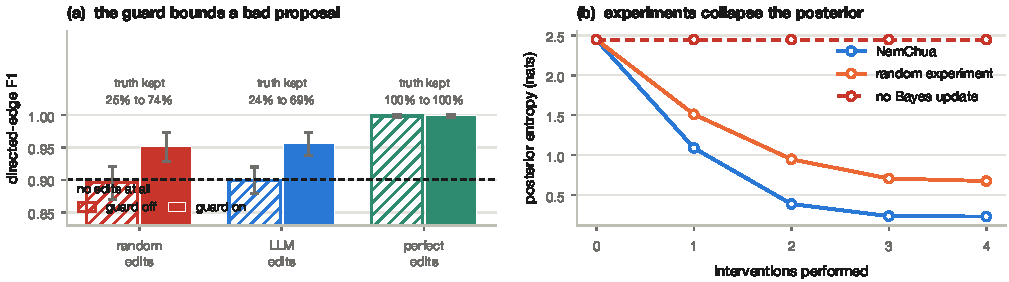
\includegraphics[width=\linewidth]{nemchua_f4_mechanism.pdf}
\caption{(a) In these runs, the guard leaves the oracle-edit arm unchanged and protects the
imperfect edit arms; annotations show how often the true DAG survives the candidate cap. (b)
Entropy of the normalized model weights. Without the likelihood update the weights never absorb
experimental evidence.}
\label{fig:mechanism}
\end{figure}

\subsection{Boundary conditions for useful proposal content}
\label{sec:when}

The near-null contrast between learned and random proposals describes the regimes we tested rather
than a universal limit on proposer value, and varying the observational sample reveals one plausible
boundary of that result. As the sample grows from $40$ to $1000$ rows, PC becomes progressively more
reliable, and
a language model separates from the random editor only at the smallest sample size; from $60$ rows
onward, the contrast is not distinguishable from zero (Figure~\ref{fig:when}(a)). This pattern is
consistent with a diminishing opportunity for proposal content: once the statistical estimator has
already recovered most adjacencies, even a better edit policy has little structure left to repair.
The fixed-cap, single-draw random control prevents a causal attribution of that interaction, but the
sweep identifies estimator error as a more informative axis than graph size alone.

Semantic context creates a second, conceptually different boundary because it can provide information
that is absent from the observational summary. We re-parameterize five published DAGs as
linear-Gaussian models and present every instance either with anonymous labels
$X_0 \dots X_{d-1}$ or with the published labels and a one-sentence domain description. The graph,
parameters, samples, and node indices remain paired across the two presentations. With only
$60$ observational rows, four of five models produce more precise edits in the semantic condition,
and \texttt{gemini-3-flash} exceeds the shared random control by $0.080$ final F1; once the sample
increases to $300$ rows, the pattern largely recedes. The contrast is therefore compatible with a
substitution effect in which prompt context is useful precisely when statistical evidence is weak.

That interpretation remains provisional because the experiment does not isolate transferable domain
knowledge. Variable labels and the domain description change together, all five networks are widely
published and may be represented in pretraining data, and the same base parameterizations recur
across models. Treating all $300$ model-instance pairs as independent would consequently overstate
the precision of the comparison. Without shuffled-label controls, separate label and description
factors, and inference clustered by base parameterization, the defensible conclusion is that semantic
prompt context can coincide with better proposals in a scarce-data regime, not that the models have
demonstrated general causal knowledge.

The oracle-edit arm provides an important counterpoint to these qualifications because it remains
substantially above both learned and random proposers and nearly reaches the graph oracle in the main
regime, demonstrating that correct adjacency repair can influence the final answer under the same
decision architecture. The negative result is thus not a claim that proposal quality is irrelevant.
Rather, it shows that the implemented interface and decision layer convert only a small fraction of
the available proposal advantage into downstream accuracy.

\begin{figure}[t]
\centering
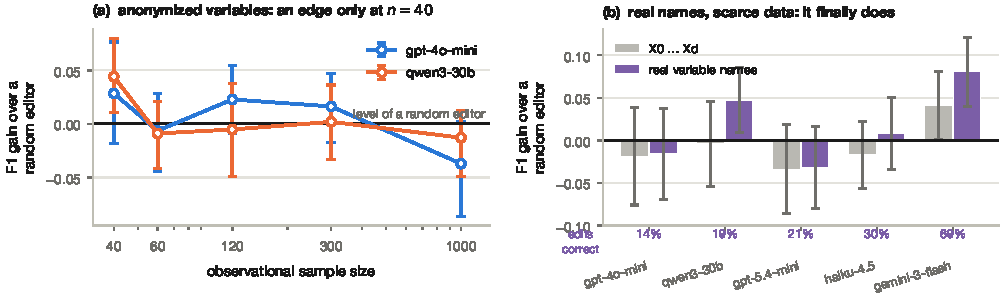
\includegraphics[width=\linewidth]{nemchua_f5_when.pdf}
\caption{Both panels are measured against the random-edit control, so zero means ``no better than
proposing at random''. (a) Anonymized synthetic instances across sample sizes. (b) Published DAG
structures at $n_{\mathrm{obs}}{=}60$, under anonymous or semantic prompt context; percentages give
edit precision in the semantic condition. This panel is exploratory because labels and description
change together and the published structures may be memorized.}
\label{fig:when}
\end{figure}

\section{Conclusion}
\label{sec:conclusion}

\nem{} succeeds as an active causal discovery system, but the attribution audit changes what that
success means. Replacing the learned proposer with cap-matched random edits nearly reproduces the
final score, while models with substantially different edit precision converge to similar answers.
The intermediate diagnostics explain this compression: better proposals improve candidate coverage,
yet bounded enumeration and approximate scoring often fail to convert that coverage into a different
submitted graph. Most of the measured advantage instead comes from the likelihood update and from
preserving unedited orientations when proposals are unreliable.

This result does not imply that proposal content is intrinsically unimportant. Oracle corrections
nearly solve the task under the same architecture, and semantic context coincides with a larger model
advantage when observational evidence is scarce. Those observations identify the conditions a useful
proposal channel must satisfy: the estimator must leave recoverable error, the proposer must receive
valid complementary evidence, candidate construction must preserve the resulting hypotheses, and the
decision layer must recognize them. The present system leaves capacity unused at several of these
links, while the misspecified partial-correlation prompt and the confounded semantic condition prevent
a broader claim about LLM causal knowledge.

System performance and generator contribution therefore require separate evaluation. Holding the
pipeline fixed while comparing no-proposal, random-proposal, and oracle-proposal controls exposes
what an end-to-end baseline cannot. In this setting, those controls show that scaffolding explains
reliability more consistently than model choice, illustrating why attribution should be measured
directly rather than inferred from system accuracy.

\appendix

\section{Formal background}
\label{app:background}

\paragraph{Causal model and identifiability.}
A linear-Gaussian structural causal model over a DAG $G$ on $d$ nodes sets
$X_j = \sum_{i \in \mathrm{pa}_G(j)} \beta_{ij}X_i + \varepsilon_j$, with independent noise
$\varepsilon_j \sim \mathcal{N}(0,\sigma_j^2)$ under assumptions of causal sufficiency,
faithfulness, and full observability. Two DAGs are Markov equivalent exactly when they share a
skeleton and the same
unshielded colliders, where $i \to k \leftarrow j$ and $i,j$ are non-adjacent. A CPDAG represents
this class by directing edges compelled in every member and leaving the remaining orientations
undetermined, so observational data identify $G$ only up to that equivalence class. A hard
intervention $\mathrm{do}(X_a=v)$ replaces the structural equation for $a$ with a constant and
deletes edges entering $a$. For a variable $X_b$ adjacent to $a$, the mean of $X_b$ under the
intervention differs from its observational mean when $a \to b$ and $v$ differs from
$\mathbb{E}[X_a]$, and is unchanged when $b \to a$; with coefficients bounded away from zero this
holds for every adjacency, which is the local evidence used to resolve orientation. Non-adjacent
descendants of $a$ also shift, so the signal is not confined to children --- what is specific to
children is that the shift is not mediated by another intervened-on path.

\paragraph{Scoring, experimental design, and evaluation.}
For each candidate $h$, we fit parameters by least squares and compute
$\mathrm{BIC}_h=-2\ell_h+k_h\log n$, normalizing
$w_h \propto \exp(-\tfrac12\mathrm{BIC}_h)$ into approximate model weights. Because BIC only
approximates integrated evidence, these weights are not an exact posterior under a fully specified
structure prior. Writing $H$ for the hypothesis index and $Y_a$ for the batch obtained from
$\mathrm{do}(X_a=v)$, the selected intervention is
$a_t=\arg\max_a \mathbb{H}[H]-\mathbb{E}_{Y_a}\mathbb{H}[H\mid Y_a]$, with the expectation
estimated from $12$ outcomes sampled under the fitted candidate models, with both entropy terms
defined only over the truncated finite set. We evaluate the submitted graph with directed-edge F1, which
requires both adjacency and orientation to be correct, skeleton F1, which ignores direction, and
structural Hamming distance (SHD), which counts the single-edge edits needed to recover $G$.

\section{Related work}
\label{sec:related}

Active causal discovery has approached intervention selection through coverage of a Markov
equivalence class, information-theoretic acquisition, Bayesian experimental design over candidate
structures, and learned or amortized policies. \nem's decision layer belongs to the model-based
branch of this literature and is not proposed as a new causal discovery algorithm. We use it because
its finite candidate set, explicit weights, and recorded updates expose the fate of each proposed
structural change, providing an unusually inspectable substrate for attribution.

Language models enter causal discovery at several levels of authority, ranging from local semantic
judgments to control of an experimental loop. They have been used as semantic experts for pairwise
cause-effect judgments, as priors or initializers for structure learning, as search operators over
graphs, and as agents that control the entire experimental loop. Much of this work evaluates only the
final graph on variables with meaningful names, where world knowledge may supply information absent
from a statistical learner, and rarely includes a model-free proposer while holding the downstream
procedure fixed. Our results offer a possible reconciliation of the mixed empirical picture:
semantic information may help when the observational estimate is weak, yet differences among
proposers can become invisible once a strong front-end or protective downstream filter determines the
answer. The present semantic experiment is consistent with this account but cannot identify it.

The same attribution problem arises wherever a generator is evaluated only after a strong filter has
acted. Program synthesis, theorem proving, and reasoning-with-verifiers all generate candidates
cheaply and rely on trusted machinery to select among them, while success is usually measured at the
boundary of the assembled system. Estimating the generator's marginal contribution is difficult when
individual proposals have no observable ground truth. Synthetic causal discovery is unusual in
providing both edit-level labels and a final task score, which allows proposal quality to be separated
from the quality of the answers produced after filtering.

\section{Instances, models and the difficulty ladder}
\label{app:instances}

Instances are sampled and filtered by a fixed acceptance policy, identical for every arm. A
candidate is rejected if its CPDAG leaves fewer than two undirected edges, if every undirected edge
meets the same node, if the skeleton is disconnected, if no intervention is needed, or if any
relevant structural partial correlation falls below a faithfulness margin of $0.1$. Edge weights
are drawn from $(-2,-0.5) \cup (0.5,2)$ with unit noise variance.

The five proposers are \texttt{qwen/qwen3-coder-30b-a3b-instruct},
\texttt{openai/gpt-4o-mini-2024-07-18}, \texttt{openai/gpt-5.4-mini},
\texttt{anthropic/claude-haiku-4.5} and \texttt{google/gemini-3-flash-preview}, all served through
OpenRouter at temperature zero. This range is intended to create meaningful variation in proposal
behavior rather than to support provider-level claims, since the models differ simultaneously in
scale, training data, and instruction tuning.

Density is $|E| = d$ by design, which calibrates PC to be competent but imperfect. At higher
density ($|E| \approx 1.4d$) PC's skeleton is wrong so often that every arm is capped at the same
low ceiling and no experiment helps. This is a limitation of the instance design rather than a
claim about dense causal discovery.

\begin{table}[h]
\caption{The difficulty ladder at $n_{\mathrm{obs}}{=}300$. $|I^*|$ is a minimum identifying
intervention set; budget is $|I^*| + 1$. Means over the twenty accepted instances per level.}
\label{tab:levels}
\centering
\small
\begin{tabular}{ccccccc}
\toprule
Level & $d$ & $|E|$ & undirected edges in CPDAG & $|I^*|$ & budget & PC skeleton F1 \\
\midrule
0 & 4  & 4  & $4.0$ & $1.5$ & $2.5$ & $0.909$ \\
1 & 6  & 6  & $3.3$ & $1.7$ & $2.7$ & $0.973$ \\
2 & 8  & 8  & $3.7$ & $1.8$ & $2.8$ & $0.967$ \\
3 & 10 & 10 & $4.2$ & $1.9$ & $2.9$ & $0.940$ \\
\bottomrule
\end{tabular}
\end{table}

The semantic study uses five small networks from the bnlearn repository: \texttt{cancer}
($d{=}5$), \texttt{earthquake} ($d{=}5$), \texttt{survey} ($d{=}6$), \texttt{asia} ($d{=}8$), and
\texttt{sachs} ($d{=}11$). We borrow their graphs and variable names and re-parameterize them as
linear-Gaussian models. The conditional distributions are ours; the structures and vocabularies
are published and may have appeared in model pretraining data.

\section{Prompts}
\label{app:prompts}

\paragraph{Proposer (system).}
\begin{quote}\small\ttfamily
You audit the adjacency structure of a causal graph estimated from a small sample. The world is an
unknown linear-Gaussian DAG with no hidden confounders and full observability. You are given the
correlation matrix, the partial correlation of every pair given all other variables, and the
adjacency set the PC algorithm returned from the same sample. Read the statistics like this: for a
linear-Gaussian DAG, two variables are directly connected if and only if their partial correlation
given all others is non-zero. So a pair with a sizeable partial correlation that PC left
non-adjacent is a likely FALSE NEGATIVE, and a pair PC made adjacent whose partial correlation is
near zero is a likely FALSE POSITIVE. With a small sample PC's independence tests are underpowered,
so borderline values matter. List only the pairs you would genuinely bet on; an empty list is a
valid and often correct answer. Do not restate the whole graph; report edits only. At most 4
removals and 4 additions. Call propose\_skeleton\_edits exactly once.
\end{quote}

\textbf{Post hoc statistical audit.} The ``if and only if'' sentence in the executed prompt is
incorrect for general DAGs. Conditioning on every remaining variable can open collider paths, so
full-order partial correlation may encode an edge of the moral graph rather than an adjacency in
the DAG. We reproduce the prompt because changing it in the paper without rerunning the proposer
would misdescribe the experiment. A valid follow-up should expose separating sets or conditional
independence evidence over multiple conditioning sets and rerun the central proposal arms.

In the semantic condition one sentence is appended: \texttt{The variables are named, and the names
are meaningful: they come from \{domain\}. Use what you know about this domain alongside the
statistics; a pair that is implausible on domain grounds is a good removal candidate even when the
statistics are borderline, and vice versa.} This condition changes both labels and a domain
description, despite the internal run label \texttt{named}.

\paragraph{User payload and output validation.}
The user message is a JSON object containing the variable list and an observational summary with the
row count, marginal moments, correlation matrix, full-order partial-correlation matrix, PC adjacency
list, and currently non-adjacent pairs. Returned skeleton edits are coerced to integer pairs,
range-checked, de-duplicated, and retained only when a removal names a current adjacency or an
addition names a current non-adjacency, while acyclicity is enforced later as each edited skeleton
is oriented. Complete-graph outputs pass through a separate sanitizer that removes self-loops,
duplicates, and conflicting edges and skips directed edges that would create a cycle. When a tool
call is malformed, the model receives at most two repair attempts before the episode continues.
Because the proposal audit in Section~\ref{sec:credit} scores edits after this filtering, it measures
the changes that candidate construction actually received rather than unexecutable text emitted by
the model.

\paragraph{End-to-end baseline.}
For completeness, the end-to-end system prompt states that the target is a directed acyclic graph,
that observational data identify only a Markov equivalence class, and that interventions should be
used to resolve directions. It explicitly says: \texttt{Use undirected\_edges only for genuinely
unresolved adjacencies.} The model receives all observational rows, the remaining budget, and the
mean and standard deviation of every collected interventional batch, and its tool call is validated
before execution. Across the $80$ \texttt{gpt-4o-mini} episodes in Table~\ref{tab:main}, all calls
are valid and none triggers a parser repair, yet every final call contains an empty
\texttt{directed\_edges} list. A representative output submits
\texttt{undirected\_edges=[[0,1],[1,2],[2,3]]} while its rationale describes $X_0$ as influencing
$X_1$ and $X_1$ as influencing $X_2$. Thus the zero directed F1 is a model behavior under this
prompt, not silent rejection by the output sanitizer.

\section{What each proposer actually proposes}
\label{app:edits}

Aggregate edit precision obscures an important asymmetry between removing and adding adjacencies.
The former chooses from PC's estimated skeleton, where spurious edges are rare, whereas the latter
searches its much larger complement for genuine omissions. We therefore evaluate removals and
additions separately against the chance rate of their respective admissible sets
(Figure~\ref{fig:a1} and Table~\ref{tab:decomp}).

The decomposition reveals that proposer quality is expressed primarily as restraint, with lower edit
volume corresponding monotonically to higher overall precision across the five models:
\texttt{gpt-4o-mini} proposes $6.4$ changes per instance and is correct $7.9\%$ of the time, whereas
\texttt{gemini-3-flash} proposes $3.0$ and is correct $32.8\%$ of the time
(Figure~\ref{fig:a1}(c)). Most of this separation comes from restraint in proposing removals because
PC introduces only about $0.1$ spurious adjacency per instance, leaving little genuine opportunity
for deletion, yet the
least selective models attempt $3.3$--$3.7$ removals while \texttt{gemini-3-flash} attempts $0.4$.
Additions present a less hostile base rate because PC misses about $1.75$ true adjacencies; every
model exceeds chance on this action and the between-model spread is correspondingly smaller. Better
proposers thus appear to understand when the evidence is too weak to justify changing an already
competent statistical estimate, even though that selectivity does not reliably improve the final
graph.

\begin{figure}[h]
\centering
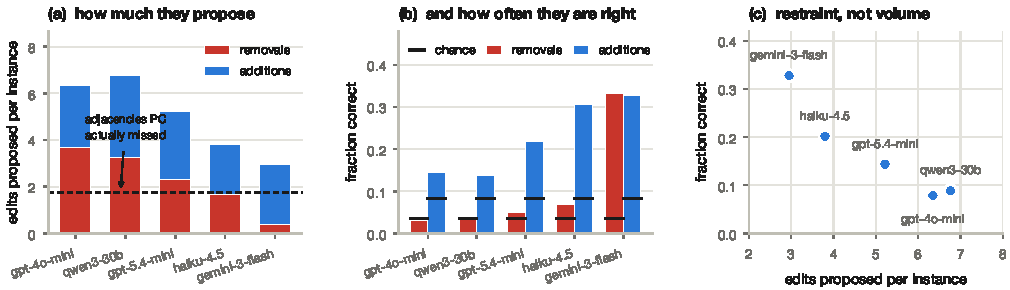
\includegraphics[width=\linewidth]{nemchua_a1_edits.pdf}
\caption{Proposal behaviour at $n_{\mathrm{obs}}{=}60$, $60$ instances per model. (a) Volume and
composition against the number of adjacencies PC actually missed. (b) Precision of each kind of
edit against the chance rate for that kind. (c) The two are strongly and negatively related.}
\label{fig:a1}
\end{figure}

\begin{table}[h]
\caption{Edit decomposition, $n_{\mathrm{obs}}{=}60$. ``Chance'' is the rate an editor drawing
uniformly from the same set would achieve: PC's spurious adjacencies as a share of its adjacency
set, and its missed adjacencies as a share of the non-adjacent pairs. ``Recall'' is the share of
PC's missed adjacencies the model proposed.}
\label{tab:decomp}
\centering
\small
\setlength{\tabcolsep}{4.5pt}
\begin{tabular}{lcccccccc}
\toprule
& \multicolumn{3}{c}{removals} & \multicolumn{3}{c}{additions} & \multicolumn{2}{c}{overall} \\
\cmidrule(lr){2-4}\cmidrule(lr){5-7}\cmidrule(lr){8-9}
Model & per inst. & correct & chance & per inst. & correct & chance & recall & correct \\
\midrule
gpt-4o-mini    & $3.68$ & $0.032$ & $0.035$ & $2.67$ & $0.144$ & $0.083$ & $0.22$ & $0.079$ \\
qwen3-30b      & $3.25$ & $0.036$ & $0.035$ & $3.52$ & $0.137$ & $0.083$ & $0.28$ & $0.089$ \\
gpt-5.4-mini   & $2.30$ & $0.051$ & $0.035$ & $2.92$ & $0.217$ & $0.083$ & $0.36$ & $0.144$ \\
haiku-4.5      & $1.68$ & $0.069$ & $0.035$ & $2.12$ & $0.307$ & $0.083$ & $0.37$ & $0.202$ \\
gemini-3-flash & $0.40$ & $0.333$ & $0.035$ & $2.55$ & $0.327$ & $0.083$ & $0.48$ & $0.328$ \\
\bottomrule
\end{tabular}
\end{table}

\section{Where the signal stops}
\label{app:chain}

The aggregate result in Section~\ref{sec:credit} can be understood only by separating the opportunity
to include a good graph from the ability to select it. Recording every intermediate object allows us
to follow five links from edit precision to the final submission (Figure~\ref{fig:a2}). Precision,
recall of PC's missing adjacencies, and the probability that the true DAG enters the candidate set all
improve with proposer quality. The best F1 available within that set rises much less, however, and
achieved F1 no longer orders the models. This divergence is the empirical basis for distinguishing
candidate coverage from downstream conversion.

\begin{figure}[h]
\centering
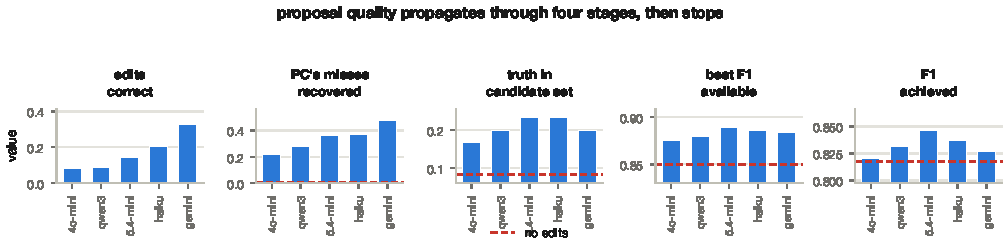
\includegraphics[width=\linewidth]{nemchua_a2_chain.pdf}
\caption{The five measurable links from proposal to answer, at $n_{\mathrm{obs}}{=}60$; models
ordered by edit precision. Dashed line is the no-edit arm. Note the changing $y$ scales: the
first three panels span a factor of four, the last two a few percent.}
\label{fig:a2}
\end{figure}

\begin{table}[h]
\caption{The five proposers in full. $\Delta$ columns are paired differences against the no-edit
and random-edit arms on the same instances; ``LLM-graphs'' is the same model asked for whole DAGs
instead of edits. $60$ instances per cell ($d \in \{6,8,10\}$).}
\label{tab:models}
\centering
\small
\setlength{\tabcolsep}{4.5pt}
\begin{tabular}{lccccccc}
\toprule
Model & edits correct & \nem{} F1 & $\Delta$ no edits & $\Delta$ random & LLM-graphs & tokens \\
\midrule
\multicolumn{7}{l}{\emph{$n_{\mathrm{obs}} = 60$; no edits $0.818$, random $0.830$, oracle edits $0.988$}}\\
gpt-4o-mini    & $0.079$ & $0.820 \pm 0.042$ & $+0.002$ & $-0.010$ & $0.582$ & $1{,}254$ \\
qwen3-30b      & $0.089$ & $0.832 \pm 0.037$ & $+0.014$ & $+0.002$ & $0.599$ & $2{,}115$ \\
gpt-5.4-mini   & $0.144$ & $0.846 \pm 0.036$ & $+0.029^{**}$ & $+0.017$ & $0.648$ & $1{,}366$ \\
haiku-4.5      & $0.202$ & $0.837 \pm 0.036$ & $+0.020^{*}$ & $+0.007$ & $0.671$ & $2{,}138$ \\
gemini-3-flash & $0.328$ & $0.827 \pm 0.037$ & $+0.009$ & $-0.003$ & $0.668$ & $1{,}560$ \\
\midrule
\multicolumn{7}{l}{\emph{$n_{\mathrm{obs}} = 300$; no edits $0.929$, random $0.929$, oracle edits $0.995$}}\\
gpt-4o-mini    & $0.037$ & $0.950 \pm 0.020$ & $+0.021$ & $+0.021$ & $0.712$ & $1{,}255$ \\
qwen3-30b      & $0.031$ & $0.937 \pm 0.026$ & $+0.008$ & $+0.008$ & $0.742$ & $2{,}061$ \\
gpt-5.4-mini   & $0.059$ & $0.939 \pm 0.027$ & $+0.010$ & $+0.009$ & $0.818$ & $1{,}355$ \\
haiku-4.5      & $0.068$ & $0.943 \pm 0.025$ & $+0.014$ & $+0.013$ & $0.824$ & $2{,}154$ \\
gemini-3-flash & $0.126$ & $0.925 \pm 0.035$ & $-0.004$ & $-0.005$ & $0.847$ & $1{,}534$ \\
\bottomrule
\end{tabular}
\end{table}

The whole-graph arm provides a complementary test because it removes the statistical skeleton as an
anchor and allows model output to define the candidate set. Under this greater authority, final
scores follow the proposal-quality ranking, rising from $0.582$ to $0.671$ at
$n_{\mathrm{obs}}{=}60$ and from $0.712$ to $0.847$ at $300$, while nevertheless remaining below
the corresponding edit-interface score in every case. Model capability is therefore easier to observe when
the model controls the hypothesis space, but the resulting system is less accurate because it also
loses the protection supplied by the statistical estimate. The edit interface masks some genuine
between-model differences as the price of making the assembled system robust to poor generations.

\section{The semantic study in full}
\label{app:semantic}

The semantic experiment asks whether a proposer becomes more useful when its prompt contains a
source of information that the anonymous correlation matrices omit. Each linear-Gaussian sample is
paired across presentations, but the semantic version restores both published variable labels and a
short domain description. The tables below retain the per-structure variation because a pooled mean
would conceal how strongly the apparent benefit depends on the identity of the benchmark network.

\begin{figure}[h]
\centering
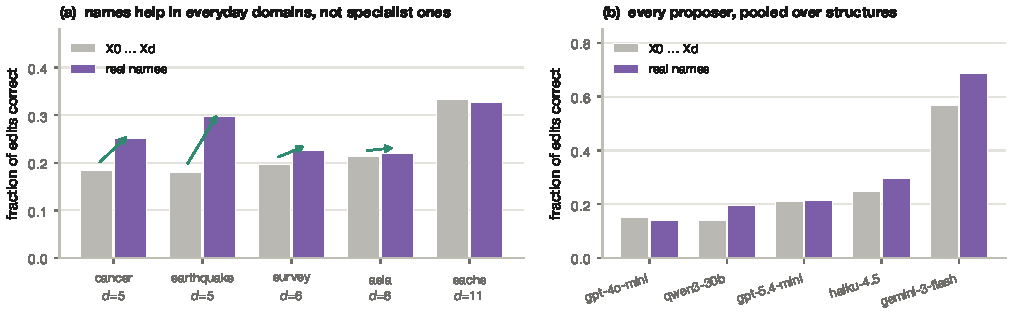
\includegraphics[width=\linewidth]{nemchua_a3_semantic.pdf}
\caption{Semantic against anonymous prompt context at $n_{\mathrm{obs}}{=}60$, with $12$
parameterizations per structure. The semantic condition changes published labels and a domain
sentence together. Panels pool over proposers or structures for visualization, not for an
independence-based significance claim.}
\label{fig:a3}
\end{figure}

\begin{table}[h]
\caption{Per-structure descriptive results at $n_{\mathrm{obs}}{=}60$, pooled over the five
proposers. Repeated parameterizations across models are not independent experimental units.}
\label{tab:semantic}
\centering
\small
\setlength{\tabcolsep}{4.5pt}
\begin{tabular}{lccccccccc}
\toprule
& & & \multicolumn{3}{c}{no-model arms} & \multicolumn{2}{c}{edits correct} & \multicolumn{2}{c}{\nem{} F1} \\
\cmidrule(lr){4-6}\cmidrule(lr){7-8}\cmidrule(lr){9-10}
Structure & $d$ & $|E|$ & PC skel. & no edits & oracle & anon. & sem. & anon. & sem. \\
\midrule
cancer     & $5$  & $4$  & $0.721$ & $0.721$ & $0.991$ & $0.183$ & $0.250$ & $0.773$ & $0.813$ \\
earthquake & $5$  & $4$  & $0.721$ & $0.721$ & $0.991$ & $0.180$ & $0.296$ & $0.756$ & $0.854$ \\
survey     & $6$  & $6$  & $0.752$ & $0.668$ & $1.000$ & $0.197$ & $0.226$ & $0.705$ & $0.673$ \\
asia       & $8$  & $8$  & $0.783$ & $0.760$ & $1.000$ & $0.213$ & $0.220$ & $0.762$ & $0.783$ \\
sachs      & $11$ & $17$ & $0.617$ & $0.391$ & $0.487$ & $0.333$ & $0.326$ & $0.410$ & $0.403$ \\
\bottomrule
\end{tabular}
\end{table}

The descriptive gain is largest on \texttt{earthquake} and \texttt{cancer}, whose labels denote
everyday concepts, and is absent on \texttt{sachs}, whose variables are signaling proteins. This is
compatible with accessible semantic associations, but it is equally compatible with different
benchmark exposure across networks; the present design cannot choose between them. A separate
computational limit becomes visible on \texttt{sachs}, where even oracle edits fail to rescue the
pipeline once the $17$-edge orientation space must be sampled rather than enumerated, since a
corrected skeleton no longer guarantees that the retained set contains the true DAG. Semantic
proposal quality and candidate-search scalability are therefore distinct bottlenecks that happen to
coincide on this network.

\section{Scaling, and the full ladder}
\label{app:scaling}

Two axes determine whether the edit interface has room to help. Increasing the observational sample
strengthens the PC estimate, while increasing graph size expands the orientation space that must fit
inside a fixed candidate budget. We examine these effects separately across sample sizes and report
each of the four main-run levels rather than relying on a pooled score
(Figure~\ref{fig:a4} and Table~\ref{tab:levels_full}).

\begin{figure}[h]
\centering
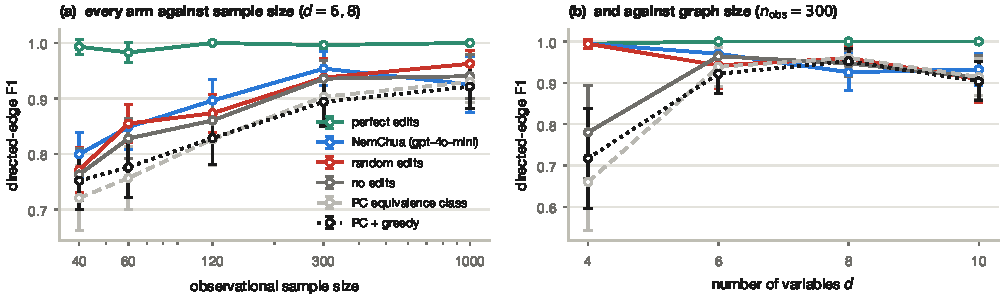
\includegraphics[width=\linewidth]{nemchua_a4_ladder.pdf}
\caption{Every arm across the two axes we vary. (a) Observational sample size at $d \in \{6,8\}$.
(b) Graph size at $n_{\mathrm{obs}}{=}300$. Oracle edits are near-flat on both axes; everything
else rises with the strength of the statistical front-end.}
\label{fig:a4}
\end{figure}

\begin{table}[h]
\caption{Per-level means from the main run, $20$ instances per cell. The edit channel pays off at
$d{=}4$, where PC's skeleton is weakest, and is otherwise roughly flat for both the random editor
and the language models. Oracle edits gain at every size.}
\label{tab:levels_full}
\centering
\small
\setlength{\tabcolsep}{6pt}
\begin{tabular}{lcccc}
\toprule
Arm & $d{=}4$ & $d{=}6$ & $d{=}8$ & $d{=}10$ \\
\midrule
PC skeleton F1 (front-end quality) & $0.909$ & $0.973$ & $0.967$ & $0.940$ \\
truth in PC's equivalence class    & $0.30$  & $0.65$  & $0.55$  & $0.30$ \\
\midrule
LLM end-to-end (qwen3-30b)   & $0.314$ & $0.211$ & $0.158$ & $0.127$ \\
LLM writes the DAG (gpt-4o-mini) & $0.476$ & $0.690$ & $0.759$ & $0.671$ \\
PC $+$ greedy $+$ \textsc{Meek} & $0.717$ & $0.922$ & $0.952$ & $0.903$ \\
PC equivalence class          & $0.660$ & $0.939$ & $0.960$ & $0.914$ \\
no edits                      & $0.780$ & $0.964$ & $0.947$ & $0.913$ \\
random edits                  & $0.994$ & $0.942$ & $0.960$ & $0.909$ \\
\nem{} (gpt-4o-mini)          & $0.994$ & $0.970$ & $0.926$ & $0.932$ \\
\nem{} (qwen3-30b)            & $0.944$ & $0.987$ & $0.949$ & $0.931$ \\
oracle edits                  & $0.994$ & $1.000$ & $1.000$ & $1.000$ \\
\bottomrule
\end{tabular}
\end{table}

The $d{=}4$ level explains most of the apparent advantage over the classical baseline even though it
contains the smallest graphs, because PC happens to have its lowest skeleton F1 there and thus leaves
the largest correctable error relative to problem size. At the larger main-run levels, the random and
learned editors fluctuate around the unedited arm without a consistent ordering. Oracle edits remain
near perfect, confirming that the correction channel still contains useful information, while the
$d{=}12$ stress test below shows how orientation sampling eventually prevents
the retained candidate set from exploiting even a correct skeleton.

\section{Robustness across design choices}
\label{sec:robust}

The same attribution pattern survives several changes to the experimental design, although the
stress tests also expose limits of the downstream machinery. Across PC significance thresholds, the
language-model arms remain close to the random editor, and increasing the edit allowance produces no
monotone improvement. A tight intervention budget makes target selection more consequential because
the policy cannot recover from an uninformative experiment, even though the max-degree heuristic
continues to track the Monte Carlo selector. At $d{=}12$, orientation sampling prevents even oracle
edits from reliably placing high-quality graphs in the retained set. We interpret this degradation as
a scalability warning about bounded candidate construction rather than as evidence against proposal
quality, keeping this failure mode separate from the quality of the proposed edits.

\begin{table}[h]
\caption{Robustness across front-end thresholds, intervention budget, and graph size. The
language-model contrast stays close to the shared random editor where both are available. Under a
tight budget, experiment selection becomes more consequential.}
\label{tab:robust}
\centering
\small
\setlength{\tabcolsep}{4.5pt}
\begin{tabular}{lccccc}
\toprule
Setting & PC skel.\ F1 & no edits & random edits & \nem{} & LLM $-$ random \\
\midrule
$\alpha = 0.01$, $n_{\mathrm{obs}}{=}60$ & $0.810$ & $0.773$ & $0.762$ & $0.782$ & $+0.015$, $+0.025$ (n.s.) \\
$\alpha = 0.05$, $n_{\mathrm{obs}}{=}60$ & $0.873$ & $0.828$ & $0.855$ & $0.847$ & $-0.006$, $-0.009$ (n.s.) \\
$\alpha = 0.10$, $n_{\mathrm{obs}}{=}60$ & $0.885$ & $0.839$ & $0.860$ & $0.852$ & $-0.022$, $+0.006$ (n.s.) \\
\midrule
tight budget (slack $0$) & $0.947$ & $0.874$ & n/a & $0.916$ & n/a \\
$d = 12$, ten instances & $0.941$ & $0.871$ & $0.870$ & $0.930$ & $+0.052$, $+0.067$ (n.s.) \\
\bottomrule
\end{tabular}
\end{table}

\section{The guard, in full}
\label{app:guard}

The guard is intended to help only when an edited neighborhood would otherwise displace useful
orientations of PC's original skeleton. The three regimes in Table~\ref{tab:guard} exhibit precisely
that pattern: imperfect proposal arms generally retain the true DAG more often and achieve higher F1
when the reservation is active. The oracle-edit arm is nearly unchanged and occasionally slightly
worse because some reserved slots are spent on a skeleton that no longer needs repair. These results
motivate the guard as a hedge against fallible proposals, while stopping short of claiming that it is
cost-free for every correct proposer, graph family, or candidate budget.

\begin{table}[h]
\caption{Guard on against guard off, paired. ``Truth kept'' is the fraction of instances whose
true DAG survives in the candidate set.}
\label{tab:guard}
\centering
\small
\setlength{\tabcolsep}{5pt}
\begin{tabular}{llcccc}
\toprule
Regime & Proposal & guard on & guard off & $\Delta$ & truth kept (on $\to$ off) \\
\midrule
\multirow{4}{*}{$n_{\mathrm{obs}}{=}60$}
 & random         & $0.855$ & $0.814$ & $+0.041^{*}$ & $0.23 \to 0.12$ \\
 & gpt-4o-mini    & $0.822$ & $0.791$ & $+0.031^{*}$ & $0.23 \to 0.12$ \\
 & qwen3-30b      & $0.836$ & $0.823$ & $+0.013$     & $0.28 \to 0.20$ \\
 & oracle         & $0.983$ & $0.991$ & $-0.008$     & $0.97 \to 1.00$ \\
\midrule
\multirow{4}{*}{$n_{\mathrm{obs}}{=}300$}
 & random         & $0.937$ & $0.892$ & $+0.045^{***}$ & $0.68 \to 0.10$ \\
 & gpt-4o-mini    & $0.963$ & $0.915$ & $+0.048^{***}$ & $0.72 \to 0.15$ \\
 & qwen3-30b      & $0.948$ & $0.894$ & $+0.054^{***}$ & $0.70 \to 0.12$ \\
 & oracle         & $0.996$ & $0.998$ & $-0.002$       & $0.97 \to 1.00$ \\
\midrule
\multirow{4}{*}{main run}
 & random         & $0.951$ & $0.895$ & $+0.056^{***}$ & $0.74 \to 0.25$ \\
 & gpt-4o-mini    & $0.956$ & $0.900$ & $+0.056^{***}$ & $0.69 \to 0.24$ \\
 & qwen3-30b      & $0.953$ & $0.907$ & $+0.046^{***}$ & $0.68 \to 0.23$ \\
 & oracle         & $0.999$ & $0.999$ & $\pm 0.000$    & $1.00 \to 1.00$ \\
\bottomrule
\end{tabular}
\end{table}

\section{Edit budget and cost}
\label{app:budget}

The edit-cap sweep tests whether the weak dependence on proposer identity is merely an artifact of a
search neighborhood that is too small. At $n_{\mathrm{obs}}{=}60$, increasing the allowance from
two to four and then eight edits produces neither a monotone improvement in final F1 nor a gain in
edit precision. Additional capacity is used mainly to propose more changes of similar quality, so it
does not address the conversion bottleneck identified in Section~\ref{sec:credit}. The random editor
at the default cap reaches $0.855$, above every LLM setting in this sweep, which further suggests
that edit volume alone cannot explain the differences among learned proposers.

\begin{table}[h]
\centering
\small
\setlength{\tabcolsep}{6pt}
\begin{tabular}{lccccccc}
\toprule
& & & \multicolumn{2}{c}{gpt-4o-mini} & \multicolumn{2}{c}{qwen3-30b} \\
\cmidrule(lr){4-5}\cmidrule(lr){6-7}
Cap & no edits & random & F1 & edits correct & F1 & edits correct \\
\midrule
2 & $0.828$ & $0.855$ & $0.818$ & $0.087$ & $0.827$ & $0.076$ \\
4 & $0.828$ & $0.855$ & $0.852$ & $0.089$ & $0.838$ & $0.089$ \\
8 & $0.828$ & $0.855$ & $0.842$ & $0.072$ & $0.831$ & $0.083$ \\
\bottomrule
\end{tabular}
\end{table}

Compute cost provides another view of the trade between model authority and downstream protection.
Placing every model-using arm on a common accuracy-versus-token plane, with model-free arms as
references, exposes the cost of repeatedly returning experimental evidence to the model
(Figure~\ref{fig:a5}). The end-to-end agent consumes roughly $30\times$ as many tokens
as \nem{} while scoring $0.75$--$0.96$ lower in F1, because each experimental batch re-enters its
context. Asking the model for whole graphs costs about as much as asking for edits but lowers F1 by
approximately $0.29$, indicating that reduced authority, rather than token count alone, accounts for
the improvement. The zero-token random editor then reaches the same region as \nem{}, separating
the efficiency of the interface from the marginal value of the learned proposal.

\begin{figure}[h]
\centering
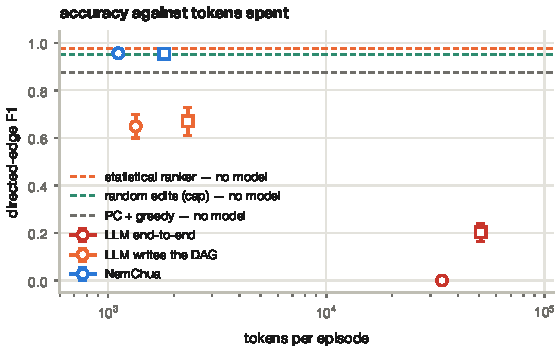
\includegraphics[width=0.52\linewidth]{nemchua_a5_cost.pdf}
\caption{Accuracy against tokens per episode on the main run. Circles are \texttt{gpt-4o-mini},
squares \texttt{qwen3-30b}.}
\label{fig:a5}
\end{figure}

\section{Additional results}
\label{app:extra}

Two near-zero ablations help delimit which architectural choices are consequential. Explicitly
adding PC's equivalence class to the edit-derived candidates changes no episode because each of its
members is already an acyclic orientation of PC's skeleton, and the guard reserves half of the
candidate budget for the best-scoring graphs of exactly that form. Similarly, submitting a graph
from edge marginals rather than selecting the highest-weight DAG reproduces the same answer under the
highly concentrated model weights, whose mean maximum is $0.93$ and whose final entropy is $0.23$
nats. These results are not independent algorithmic successes; they show that both operations are
functionally redundant within the implemented pipeline and therefore cannot explain its advantage.

The sample-size sweep below broadens the random-editor comparison beyond the default observational
regime. Each cell contains $40$ paired instances, and the reported entries are F1 differences rather
than absolute arm scores, with stars indicating two-sided Wilcoxon signed-rank results. Learned edits
do not maintain a consistent advantage as PC improves: their differences from random edits change
sign across sample sizes, whereas the oracle comparison remains positive throughout. This pattern
supports an opportunity-based interpretation in which genuine skeleton corrections retain value but
the implemented model proposals do not exploit that value reliably.

\begin{table}[h]
\caption{Paired F1 differences across observational sample sizes, with $40$ instances per cell.}
\centering
\small
\begin{tabular}{lccccc}
\toprule
$n_{\mathrm{obs}}$ & $40$ & $60$ & $120$ & $300$ & $1000$ \\
\midrule
PC skeleton F1                   & $0.824$ & $0.873$ & $0.900$ & $0.957$ & $0.968$ \\
\midrule
gpt-4o-mini $-$ random           & $+0.029$ & $-0.006$ & $+0.023$ & $+0.016$ & $-0.037$ \\
qwen3-30b $-$ random             & $+0.044^{*}$ & $-0.008$ & $-0.004$ & $+0.003$ & $-0.013$ \\
oracle edits $-$ no edits        & $+0.230^{***}$ & $+0.155^{***}$ & $+0.129^{***}$ & $+0.055^{**}$ & $+0.060^{**}$ \\
\bottomrule
\end{tabular}
\end{table}

We also corrected an enumeration asymmetry that could plausibly have hidden the models' strongest
proposal signal. The first implementation listed all removals before additions and truncated the
variant list at six, causing a proposal with four removals to lose most of its additions even though
PC omits many more true edges than it invents. We placed the all-edits variant first, interleaved
single removals and additions, raised the cap, and replayed every affected arm on identical recorded
proposals. Final F1 moved by at most $0.007$ for every model, with no significant change. The flat
capability curve in Section~\ref{sec:credit} therefore cannot be attributed to the ordering artifact,
even though correcting it makes the implemented interface better aligned with where proposal quality
is observed.

\section{Limitations}
\label{app:limitations}

\paragraph{The executed prompt contains a causal-statistical error.}
The proposer was told that full-order partial correlation characterizes DAG adjacency, an equivalence
that fails in the presence of colliders and may have systematically directed the model toward poor
edits. Consequently, the current null result applies to the executed interface rather than to an LLM
supplied with valid separating-set, stability, or multi-conditioning-set evidence. Repairing the
prompt requires rerunning the proposer arms and is the highest-priority follow-up because no textual
qualification can recover the counterfactual proposals that a statistically correct prompt would
have produced.

\paragraph{The random control is cap-matched and single-draw.}
\texttt{random-edits} draws up to four removals and four additions, matching the allowance given to
the models rather than each model's realized edit counts, and one seeded draw per instance produces
the single shared row reported throughout. This design answers whether a weak proposer can reproduce
the LLM result at the permitted edit volume, but it does not estimate a complete randomization
distribution or isolate proposal content from proposal count. Per-model controls matched separately
to realized removals and additions, repeated random draws, and a data-only edit ranker would provide
a sharper estimate of the marginal value contributed by model selection.

\paragraph{The semantic contrast is confounded.}
The semantic condition changes both variable labels and a domain description, and all five networks
are established benchmarks that may have been memorized during pretraining. Model episodes also
reuse the same base parameterizations, making episode-level observations within a base instance
dependent across proposers. The current comparison can therefore establish an association between
semantic presentation and proposal quality, but it cannot identify which source of information
caused that association. Shuffled labels, separate label and description factors, novel domain
graphs, and cluster-aware inference are required before attributing the difference to transferable
domain knowledge.

\paragraph{The decision layer is approximate and does not scale.}
BIC weights approximate model evidence, parameters are point estimates, expected information gain
uses Monte Carlo, and only $48$ candidate DAGs survive. Orientation enumeration becomes sampling at
larger $d$, allowing the filter to miss the truth even when an edit repairs the skeleton. These
approximations interact rather than fail independently: candidate omission cannot be repaired by
better intervention selection, while concentrated weights can hide the omission by expressing high
confidence only within the retained set. A large final maximum weight is therefore evidence of
concentration inside a truncated fitted model, not calibrated evidence that the selected DAG is
correct in the unrestricted graph space.

\paragraph{One model class, one front-end.}
All results assume linear-Gaussian mechanisms, causal sufficiency, full observability, hard
interventions, and a PC observational estimate. Varying sample size and PC's significance threshold
changes the amount of residual error but not its qualitative source. Other estimators, nonlinear or
non-Gaussian mechanisms, latent confounding, or soft interventions may leave a different error
pattern and alter both the value of semantic knowledge and the downstream likelihood. Transporting
our conclusions to those settings therefore requires repeating the same proposer-replacement audit.

\end{document}
